\chapter{Block encoding}

In order to perform matrix computations, we must first address the problem of the \textit{input model}: how to get access to information in a matrix $A\in\CC^{N\times N}$ ($N=2^n$) which is generally a non-unitary matrix, into the quantum computer? 
One possible input model is given via the unitary $e^{\I \tau A}$ (if $A$ is not Hermitian, in some scenarios we can consider its Hermitian version via the dilation method). 
This is particularly useful when $e^{\I \tau A}$ can be constructed using simple circuits, e.g. Trotter splitting.

A more general input model, as will be discussed in this chapter, is called ``block encoding''.
Of course, if $A$ is a dense matrix without obvious structures, any input model will be very expensive (e.g. exponential in $n$) to implement.
Therefore a commonly assumed input model is $s$-sparse, i.e., there are at most $s$ nonzero entries in each row / column of the matrix.
Furthermore, we have an efficient procedure to get access to the location, as well as the value of the nonzero entries.
This in general can again be a difficult task given that the number of nonzero entries can still be exponential in $n$ for a sparse matrix.
Some dense matrices may also be efficiently block encoded on quantum computers.
This chapter will illustrate the block encoding procedure for via a number of detailed examples. 

\section{Query model for matrix entries}

The query model for sparse matrices is based on certain quantum oracles. In some scenarios, these quantum oracles can be implemented all the way to the elementary gate level. 

Throughout the discussion we assume $A$ is an $n$-qubit, square matrix, and
\begin{equation}
\norm{A}_{\max}:=\max_{ij} \abs{A_{ij}}< 1.
\end{equation}
If the $\norm{A}_{\max}\ge1$, we can simply consider the rescaled matrix $\wt{A}/\alpha$ for some $\alpha>\norm{A}_{\max}$.

To query the entries of a matrix, the desired oracle takes the following general form
\begin{equation}
O_A \ket{0}\ket{i}\ket{j}=\left(A_{ij}\ket{0}+\sqrt{1-\abs{A_{ij}}^2}\ket{1}\right)\ket{i}\ket{j}.
\label{eqn:entry_oracle}
\end{equation}
In other words, given $i,j\in[N]$ and a signal qubit $0$, $O_A$ performs a controlled rotation (controlling on $i,j$) of the signal qubit, which encodes the information in terms of amplitude of $\ket{0}$.

However, the classical information in $A$ is usually not stored natively
in terms of such an oracle $O_A$. Sometimes it is more natural to assume that there is an oracle
\begin{equation}
\wt{O}_A\ket{0^{d'}}\ket{i}\ket{j}=\ket{\wt{A}_{ij}}\ket{i}\ket{j},
\end{equation}
where $\wt{A}_{ij}$ is a $d'$-bit fixed point representation of $A_{ij}$,
and the value of $\wt{A}_{ij}$ is either computed on-the-fly with a quantum computer, or obtained through an external database.
In either case, the implementation of $\wt{O}_A$ may be challenging, and we will only consider the query complexity with respect to this oracle.

Using \textit{classical arithmetic operations}, we can convert this oracle into an oracle
\begin{equation}
O'_A \ket{0^d}\ket{i}\ket{j}=\ket{\wt{\theta}_{ij}}\ket{i}\ket{j},
\end{equation}
where $0\le \wt{\theta}_{ij}< 1$, and $\wt{\theta}_{ij}$ is a $d$-bit representation of $\theta_{ij}=\arccos(A_{ij})/\pi$~. This step may require some additional work registers not shown here.


Now using the controlled rotation in \cref{prop:controlled_rotation}, the information of $\wt{A}_{ij}$, $\wt{\theta}_{ij}$ has now been transferred to the phase of the signal qubit. 
We should then perform uncomputation and free the work register storing such intermediate information $\wt{A}_{ij}$, $\wt{\theta}_{ij}$. The procedure is as follows 
\begin{equation}\label{eqn:matrixentry_access}
\begin{split}
\ket{0}\underbrace{\ket{0^d}}_{\text{work register}}\ket{i}\ket{j}\xrightarrow{O'_A} &\ket{0}\ket{\wt{\theta}_{ij}}\ket{i}\ket{j}\\
\xrightarrow{\opr{CR}}& \left(A_{ij}\ket{0}+\sqrt{1-\abs{A_{ij}}^2}\ket{1}\right)\ket{\wt{\theta}_{ij}}\ket{i}\ket{j}\\
\xrightarrow{(O'_A)^{-1}}& \left(A_{ij}\ket{0}+\sqrt{1-\abs{A_{ij}}^2}\ket{1}\right)\ket{0^d}\ket{i}\ket{j}
\end{split}
\end{equation}

From now on, we will always assume that the matrix entries of $A$ can be queried using the phase oracle $O_A$ or its variants.






\section{Block encoding}


The simplest example of block encoding is the following: 
assume we can find a $(n+1)$-qubit unitary matrix $U$ (i.e., $U\in\CC^{2N\times 2N}$) such that
\begin{equation*}
U_A=\begin{pmatrix}
{A} & {*} \\
{*} & {*}
\end{pmatrix}
\end{equation*}
where $*$ means that the corresponding matrix entries are irrelevant,
then for any $n$-qubit quantum state $\ket{b}$, we can consider the state
\begin{equation}
\ket{0,b}=\ket{0}\ket{b}=\begin{pmatrix}
b\\ 0
\end{pmatrix},
\end{equation}
and
\begin{equation}
U_A\ket{0,b}=\begin{pmatrix}
Ab\\
*
\end{pmatrix}
=:\ket{0}A\ket{b}+\ket{\perp}.
\end{equation}
Here the (unnormalized) state $\ket{\perp}$ can be written as $\ket{1}\ket{\psi}$ for some (unnormalized) state $\ket{\psi}$, that is irrelevant to the computation of $A\ket{b}$.
In particular, it satisfies the orthogonality relation.
\begin{equation}
(\bra{0}\otimes I_n)\ket{\perp}=0.
\end{equation}
In order to obtain $A\ket{b}$, we need to \textit{measure} the qubit $0$ and only keep the state if it returns $0$. This can be summarized into the following quantum circuit: 

\begin{figure}[H]
\begin{center}
\begin{quantikz}
  \lstick{$\ket{0}$}&  \qw & \gate[2]{U_{A}}   \qw & \meter{} \\
  \lstick{$\ket{b}$}& \qw & &\qw \rstick{$\frac{A\ket{b}}{\norm{A\ket{b}}} (\mbox{upon measuring 0})$}\\
\end{quantikz}
\end{center}
\caption{Circuit for block encoding of $A$ using one ancilla qubit.}
\label{fig:circuit_be_onequbit}
\end{figure}
Note that the output state is normalized after the measurement takes place.
The success probability of obtaining $0$ from the measurement can be computed as
\begin{equation}
p(0)=\norm{A\ket{b}}^2=\braket{b|A^{\dag}A|b}.
\end{equation}
So the missing information of norm $\norm{A\ket{b}}$ can be recovered via the success probability $p(0)$ if needed.
We find that the success probability is only determined by $A,\ket{b}$, and is independent of other irrelevant components of $U_A$.


Note that we may not need to restrict the matrix $U_A$ to be a $(n+1)$-qubit matrix. If we can find any $(n+m)$-qubit matrix $U_A$ so that
\begin{equation}
U_A=\begin{pmatrix}
A & * & \cdots & *\\
* & * & \cdots & *\\
\vdots & & \vdots\\
* & * & \cdots & *
\end{pmatrix}
\end{equation}
Here each $*$ stands for an $n$-qubit matrix, and there are $2^m$ block rows / columns in $U_A$. The relation above can be written compactly using the braket notation as
\begin{equation}
A=\left(\langle 0^m | \otimes I_n\right) U_A \left( | 0^m \rangle \otimes I_n
\right)
\end{equation}

A necessary condition for the existence of $U_A$ is that $\norm{A}\le 1$. (Note: $\norm{A}_{\max}\le 1$ does not guarantee that $\norm{A}\le 1$, see \cref{exer:A_spec_max_norm}).
However, if we can find sufficiently large $\alpha$ and $U_A$ so that
\begin{equation}
A/\alpha=\left(\langle 0^m | \otimes I_n\right) U_A \left( | 0^m \rangle \otimes I_n
\right).
\end{equation}
Measuring the $m$ ancilla qubits and all $m$-qubits return $0$, we still obtain the normalized state $\frac{A\ket{b}}{\norm{A\ket{b}}}$.
The number $\alpha$ is hidden in the success probability:
\begin{equation}
p(0^m)=\frac{1}{\alpha^2}\norm{A\ket{b}}^2=\frac{1}{\alpha^2}\braket{b|A^{\dag}A|b}.
\end{equation}
So if $\alpha$ is chosen to be too large, the probability of obtaining all $0$'s from the measurement can be vanishingly small.

Finally, it can be difficult to find $U_A$ to block encode $A$ exactly. This is not a problem, since it is sufficient if we can find $U_A$ to block encode $A$ up to some error $\epsilon$. We are now ready to give the definition of block encoding in \cref{def:blockencode}.
 



\begin{defn}[Block encoding] Given an $n$-qubit matrix $A$, if we can find $\alpha, \epsilon \in \mathbb{R}_+$, and an $(m+n)$-qubit unitary matrix $U_A$ so that 
\begin{equation}
\Vert A - \alpha \left(\langle 0^m | \otimes I_n\right) U_A \left( | 0^m \rangle \otimes I_n \right) \Vert \leq \epsilon,
\end{equation}
then $U_A$ is called an $(\alpha, m, \epsilon)$-block-encoding of $A$.
When the block encoding is exact with $\epsilon=0$, $U_A$ is called an $(\alpha, m)$-block-encoding of $A$. The set of all $(\alpha, m, \epsilon)$-block-encoding of $A$ is denoted by $\BE_{\alpha,m}(A,\epsilon)$, and we define $\BE_{\alpha,m}(A)=\BE(A,0)$.
\label{def:blockencode}
\end{defn}


Assume we know each matrix element of the $n$-qubit matrix $A_{ij}$, and we are given an $(n+m)$-qubit unitary $U_A$. In order to verify that $U_A\in\BE_{1,m}(A)$, we only need to verify that
\begin{equation}
\braket{0^m,i|U_A|0^m,j}=A_{ij},
\end{equation}
and $U_A$ applied to any vector $\ket{0^m,b}$ can be obtained via the superposition principle.

Therefore we may first evaluate the state $U_A\ket{0^m,j}$, and perform inner product with $\ket{0^m,i}$ and verify the resulting the inner product is $A_{ij}$.
We will also use the following technique frequently. Assume $U_A=U_B U_C$, and then
\begin{equation}
\braket{0^m,i|U_A|0^m,j}=\braket{0^m,i|U_B U_C|0^m,j}=(U_B^{\dag}\ket{0^m,i})^{\dag}(U_C\ket{0^m,j}).
\end{equation}
So we can evaluate the states $U_B^{\dag}\ket{0^m,i},U_C\ket{0^m,j}$ independently, and then verify the inner product is $A_{ij}$.
Such a calculation amounts to running the circuit \cref{fig:circuit_be_mqubit}, and if the ancilla qubits are measured to be $0^m$, the system qubits return the normalized state $\sum_{i}A_{ij}\ket{i}/\norm{\sum_{i}A_{ij}\ket{i}}$.
\begin{figure}[H]
\begin{center}
\begin{quantikz}
  \lstick{$\ket{0^m}$}&  \qw & \gate[2]{U_{A}}   \qw & \meter{} \\
  \lstick{$\ket{j}$}& \qw & &\qw \\
\end{quantikz}
\end{center}
\caption{Circuit for general block encoding of $A$.}
\label{fig:circuit_be_mqubit}
\end{figure}


\begin{exam}[$(1,1)$-block-encoding is general]\label{exam:be11}
For any $n$-qubit matrix $A$ with $\norm{A}_2\le 1$, the singular value decomposition (SVD) of $A$ is denoted by $W\Sigma V^{\dag}$, where all singular values in the diagonal matrix $\Sigma$ belong to $[0,1]$. Then we may construct an $(n+1)$-qubit unitary matrix
\begin{equation}
\begin{split}
U_A:=&\left(\begin{array}{cc}
W & 0 \\
0 & I_{n}
\end{array}\right)\left(\begin{array}{cc}
\Sigma & \sqrt{I_{n}-\Sigma^{2}} \\
\sqrt{I_{n}-\Sigma^{2}} & -\Sigma
\end{array}\right)\left(\begin{array}{cc}
V^{\dagger} & 0 \\
0 & I_{n}
\end{array}\right)\\
=&\left(\begin{array}{cc}
A &  W \sqrt{I_{n}-\Sigma^{2}} \\
\sqrt{I_{n}-\Sigma^{2}} V^{\dagger} & -\Sigma
\end{array}\right)\\
\end{split}
\end{equation}
which is a $(1,1)$-block-encoding of $A$. 
\end{exam}


\begin{exam}[Random circuit block encoded matrix]
In some scenarios, we may want to construct a pseudo-random non-unitary matrix on quantum computers. Note that it would be highly inefficient if we first generate a dense pseudo-random matrix $A$ classically and then feed it into the quantum computer using e.g. quantum random-access memory (QRAM). Instead we would like to work with matrices that are \emph{inherently easy} to generate on quantum computers. 
This inspires the random circuit based block encoding matrix (RACBEM) model~\cite{DongLin2021}. Instead of first identifying $A$ and then finding its block encoding $U_A$, we reverse this thought process: we first identify a unitary $U_A$ that is easy to implement on a quantum computer, and then ask which matrix can be block encoded by $U_A$. 


\cref{exam:be11} shows that in principle, any matrix $A$ with $\norm{A}_2\le 1$ can be accessed via a $(1,1,0)$-block-encoding. In other words, $A$ can be block encoded by an $(n+1)$-qubit random unitary $U_A$, and $U_A$ can be constructed using only basic one-qubit unitaries and CNOT gates.
The layout of the two-qubit operations can be designed to be compatible with the coupling map of the hardware.  A cartoon is shown in \cref{fig:racbem_cartoon}, and an example is given in \cref{fig:racbem_3qubit}.

\begin{figure}[htbp]
\begin{center}
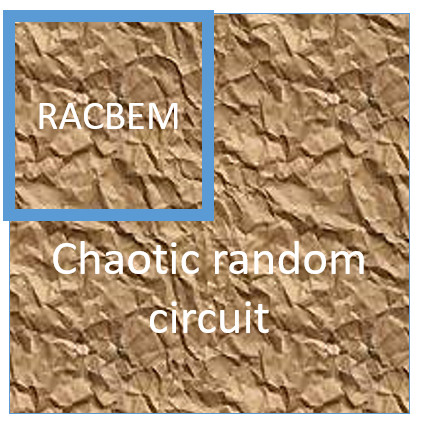
\includegraphics[width=0.2\textwidth]{racbem_cartoon.png}
\caption{A cartoon illustration of the RACBEM model.}
\end{center}
\label{fig:racbem_cartoon}
\end{figure}

\begin{figure}[htbp]
    \centering
    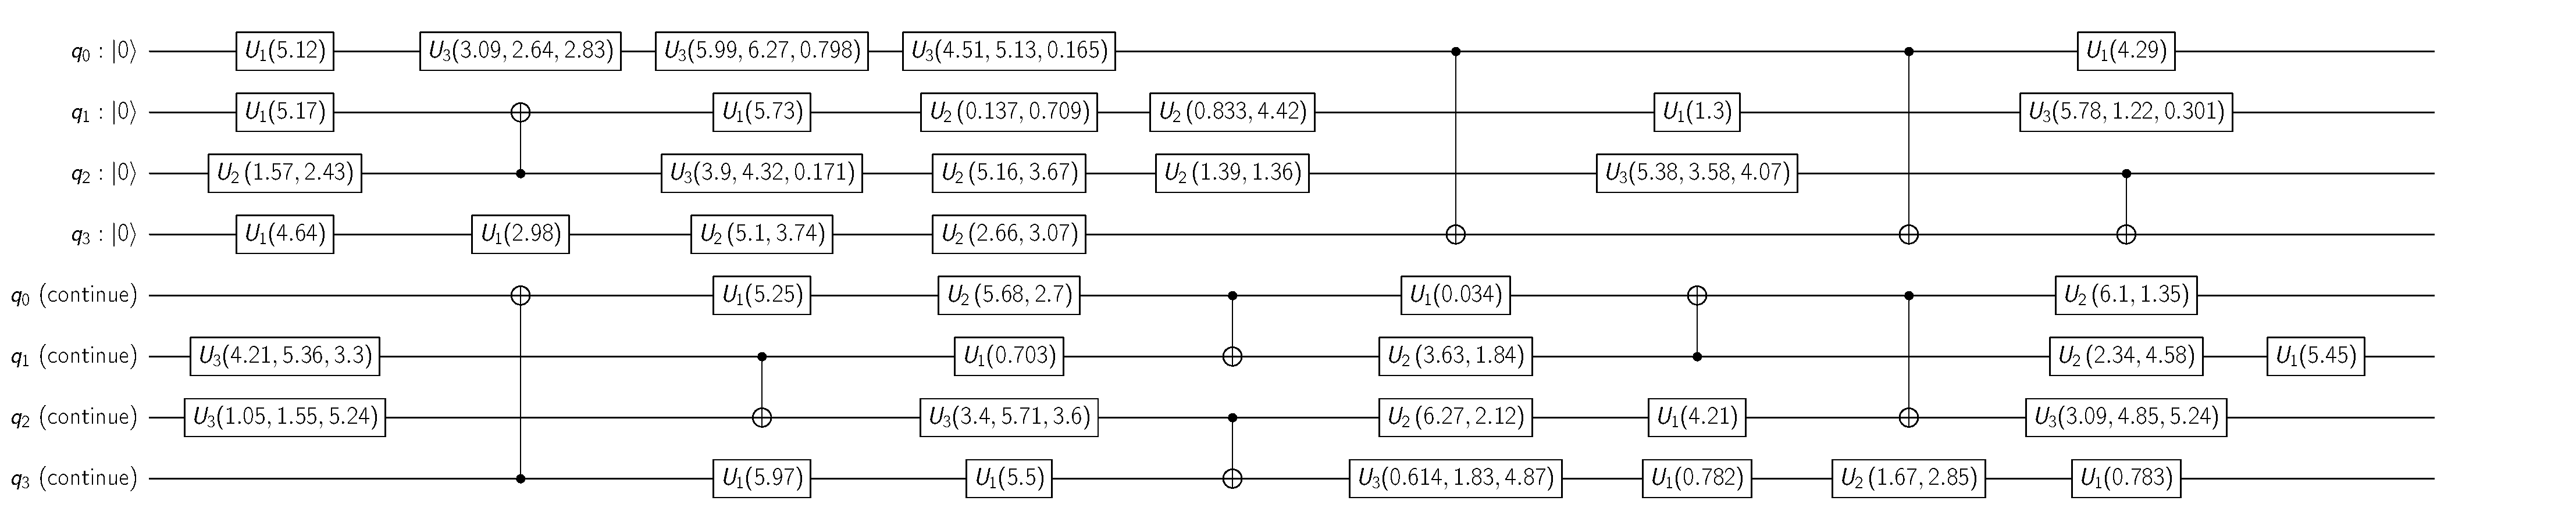
\includegraphics[width=\textwidth]{racbem_qc_nsysq_3.pdf}
    
        \centering 
        \begin{center}
            \scalebox{0.575}{$A = \left(\begin{array}{*{8}{r}}
0.096+0.256\I & -0.041+0.058\I & 0.096-0.224\I & 0.120+0.061\I & -0.138-0.054\I & 0.013+0.052\I & 0.189-0.099\I & 0.152-0.166\I \\ 
0.143-0.023\I & 0.001-0.335\I & 0.046-0.237\I & -0.056+0.007\I & 0.063+0.016\I & 0.079-0.063\I & 0.017+0.276\I & -0.046+0.007\I \\ 
0.054-0.017\I & -0.073+0.149\I & -0.002-0.063\I & -0.128+0.128\I & -0.371+0.048\I & -0.163-0.102\I & -0.069-0.069\I & 0.126+0.037\I \\ 
-0.043-0.208\I & -0.156-0.170\I & 0.189-0.080\I & -0.090+0.142\I & -0.057+0.075\I & 0.252+0.080\I & 0.150+0.057\I & 0.098-0.043\I \\ 
0.145+0.178\I & -0.325+0.125\I & 0.114+0.242\I & -0.136-0.316\I & 0.145+0.255\I & -0.120-0.335\I & -0.046+0.295\I & -0.142-0.184\I \\ 
-0.117+0.149\I & -0.101+0.338\I & -0.213-0.018\I & -0.474+0.081\I & -0.036-0.121\I & 0.444+0.147\I & -0.198+0.035\I & -0.091-0.054\I \\ 
-0.063+0.305\I & 0.001-0.145\I & -0.177+0.045\I & -0.209-0.150\I & -0.041+0.296\I & 0.046+0.082\I & 0.387-0.051\I & -0.430+0.233\I \\ 
-0.093-0.127\I & 0.254+0.307\I & -0.144-0.265\I & -0.048-0.353\I & 0.023+0.060\I & 0.085-0.156\I & 0.011+0.225\I & 0.249+0.420\I \\ 
\end{array}\right)$}
        \end{center}
    \caption{A RACBEM circuit constructed using the basic gate set $\{ \mathrm{U}_1, \mathrm{U}_2, \mathrm{U}_3, \mathrm{CNOT} \}$. The circuit at the bottom is a continuation of the top circuit.
$A$ is the 3-qubit matrix block encoded as the upper-left block, namely, identifying $q_0$ as the block encoding qubit.}
\label{fig:racbem_3qubit}
\end{figure}



\end{exam}


\begin{exam}[Block encoding of a diagonal matrix]
\label{exam:block_encode_diagonal}
As a special case, let us consider the block encoding of a diagonal matrix.
Since the row and column indices are the same, we may simplify the oracle \cref{eqn:entry_oracle} into
\begin{equation}
O_A \ket{0}\ket{i}=\left(A_{ii}\ket{0}+\sqrt{1-\abs{A_{ii}}^2}\ket{1}\right)\ket{i}.
\end{equation}
In the case when the oracle $\wt{O}_A$ is used, we may assume accordingly
\begin{equation}
\wt{O}_A \ket{0^{d'}}\ket{i}=\ket{A_{ii}}\ket{i}.
\end{equation}
Let $U_A=O_A$. Direct calculation shows that for any $i,j\in [N]$,
\begin{equation}
\bra{0}\bra{i}U_A\ket{0}\ket{j}=A_{ii}\delta_{ij}.
\end{equation}
This proves that $U_A\in\BE_{1,1}(A)$, i.e., $U_A$ is a $(1,1)$-block-encoding of the diagonal matrix $A$.
\end{exam}

\section{Block encoding of $s$-sparse matrices}

We now give a few examples of block encodings of more general sparse matrices.
We start from a $1$-sparse matrix, i.e., there is only one nonzero entry in each row or column of the matrix. This means that for each $j\in [N]$, there is a unique $c(j)\in[N]$ such that $A_{c(j),j}\ne 0$, and the mapping $c$ is a permutation. Then there exists a unitary $O_c$ such that
\begin{equation}
O_{c}\ket{j}=\ket{c(j)}.
\end{equation}
The implementation of $O_c$ may require the usage of some work registers that are omitted here. We also have
\begin{equation}
O_c^{\dag}\ket{c(j)}=\ket{j}.
\end{equation}

We assume the matrix entry $A_{c(j),j}$ can be queried via
\begin{equation}
O_A \ket{0}\ket{j}=\left(A_{c(j),j}\ket{0}+\sqrt{1-\abs{A_{c(j),j}}^2}\ket{1}\right)\ket{j}.
\end{equation}
Now we construct $U_A=(I\otimes O_c)O_A$, and compute
\begin{equation}
\bra{0}\bra{i}U_A\ket{0}\ket{j}=\bra{0}\bra{i}\left(A_{c(j),j}\ket{0}+\sqrt{1-\abs{A_{c(j),j}}^2}\ket{1}\right)\ket{c(j)}
=A_{c(j),j} \delta_{i,c(j)}.
\end{equation}
This proves that $U_A\in\BE_{1,1}(A)$.

For a more general $s$-sparse matrix, WLOG we assume each row and column has exactly $s$ nonzero entries (otherwise we can always treat some zero entries as nonzeros). 
For each column $j$, the row index for the $\ell$-th nonzero entry is denoted by $c(j,\ell)\equiv c_{j,\ell}$. 
For simplicity, we assume that there exists a unitary $O_c$ such that
\begin{equation}
O_c\ket{\ell}\ket{j}=\ket{\ell}\ket{c(j,\ell)}.
\label{eqn:Oc_sparsecol}
\end{equation}
Here we assume $s=2^\mf{s}$ and the first register is an $\mf{s}$-qubit register. 
A necessary condition for this query model is that $O_c$ is reversible, i.e., we can have $O_c^{\dag}\ket{\ell}\ket{c(j,\ell)}=\ket{\ell}\ket{j}$. This means that for each row index $i=c(j,\ell)$, we can recover the column index $j$ given the value of $\ell$. 
This can be satisfied e.g. 
\begin{equation}
c(j,\ell)=j+\ell-\ell_0 \pmod N,
\end{equation}
where $\ell_0$ is a fixed number. This corresponds to a banded matrix. 
This assumption is of course somewhat restrictive. We shall discuss more general query models in \cref{sec:query_general}. 

Corresponding to \cref{eqn:Oc_sparsecol}, the matrix entries can be queried via
\begin{equation}
O_{A}\ket{0}\ket{\ell}\ket{j}=\left(A_{c(j,\ell),j}\ket{0}+\sqrt{1-\abs{A_{c(j,\ell),j}}^2}\ket{1}\right)\ket{\ell}\ket{j}.
\end{equation}
In order to construct a unitary that encodes all row indices at the same time, we define $D=H^{\otimes \mf{s}}$ (sometimes called a diffusion operator, which is a term originated from Grover's search) satisfying
\begin{equation}
D\ket{0^{\mathfrak{s}}}=\frac{1}{\sqrt{s}}\sum_{\ell\in[s]} \ket{\ell}.
\end{equation}

Consider $U_A$ given by the circuit in \cref{fig:UA_s_sparse}.
The measurement means that to obtain $A\ket{b}$, the ancilla register should all return the value $0$.

\begin{figure}[H]
\begin{center}
\begin{quantikz}
\lstick{$\ket{0}$}&  \qw & \gate[3]{O_{A}}   & \qw& \qw & \meter{}\\
\lstick{$\ket{0^\mathfrak{s}}$}&  \gate{D} &    & \gate[2]{O_c}& \gate{D} & \meter{} \\
\lstick{$\ket{b}$}& \qw &  & & \qw & \qw
\end{quantikz}
\end{center}
\caption{Quantum circuit for block encoding an $s$-sparse matrix.}
\label{fig:UA_s_sparse}
\end{figure}

\begin{prop}
The circuit in \cref{fig:UA_s_sparse} defines $U_A\in \BE_{s,\mathfrak{s}+1}(A)$. 
\end{prop}

\begin{proof}
We call $\ket{0}\ket{0^{\mathfrak{s}}}\ket{j}$ the source state, and $\ket{0}\ket{0^{\mathfrak{s}}}\ket{i}$ the target state. In order to compute the inner product $\bra{0}\bra{0^{\mathfrak{s}}}\bra{i} U_A \ket{0}\ket{0^{\mathfrak{s}}}\ket{j}$, we apply $D,O_A,O_c$ to the source state accordingly as
\begin{equation}
\begin{split}
\ket{0}\ket{0^{\mathfrak{s}}}\ket{j}\xrightarrow{D} & \frac{1}{\sqrt{s}}\sum_{\ell\in[s]} \ket{0}\ket{\ell}\ket{j}\\
\xrightarrow{O_A} & \frac{1}{\sqrt{s}}\sum_{\ell\in[s]} \left(A_{c(j,\ell),j}\ket{0}+\sqrt{1-\abs{A_{c(j,\ell),j}}^2}\ket{1}\right)\ket{\ell}\ket{j}\\
\xrightarrow{O_c} & \frac{1}{\sqrt{s}}\sum_{\ell\in[s]} \left(A_{c(j,\ell),j}\ket{0}+\sqrt{1-\abs{A_{c(j,\ell),j}}^2}\ket{1}\right)\ket{\ell}\ket{c(j,\ell)}.
\end{split}
\end{equation}
Since we are only interested in the final state when all ancilla qubits are the $0$ state, we may apply $D$ to target state $\ket{0}\ket{0^{\mathfrak{s}}}\ket{i}$ as (note that $D$ is Hermitian)
\begin{equation}
\ket{0}\ket{0^{\mathfrak{s}}}\ket{i}\xrightarrow{D}  \frac{1}{\sqrt{s}}\sum_{\ell'\in[s]} \ket{0}\ket{\ell'}\ket{i}.
\end{equation}
Hence the inner product
\begin{equation}
\bra{0}\bra{0^{\mathfrak{s}}}\bra{i} U_A \ket{0}\ket{0^{\mathfrak{s}}}\ket{j}=\frac{1}{s}\sum_{\ell}A_{c(j,\ell),j} \delta_{i,c(j,\ell)}=\frac{1}{s}A_{ij}.
\end{equation}
\end{proof}


\section{Hermitian block encoding}\label{sec:herm_be}

So far we have considered general $s$-sparse matrices. 
Note that if $A$ is a Hermitian matrix, its $(\alpha, m, \epsilon)$-block-encoding $U_A$ does not need to be Hermitian. 
Even if $\epsilon=0$, we only have that the upper-left $n$-qubit block of $U_A$ is Hermitian. 
For instance, even the block encoding of a Hermitian, diagonal matrix in \cref{exam:block_encode_diagonal} may not be Hermitian (exercise).
On the other hand, there are indeed cases when $U_A=U_A^{\dag}$ is indeed a Hermitian matrix, and hence the definition:


\begin{defn}[Hermitian block encoding] Let $U_A$ be an $(\alpha, m, \epsilon)$-block-encoding of $A$. If $U_A$ is also Hermitian, then it is called an  $(\alpha, m, \epsilon)$-Hermitian-block-encoding of $A$. When $\epsilon=0$, it is called an $(\alpha, m)$-Hermitian-block-encoding.
The set of all $(\alpha, m, \epsilon)$-Hermitian-block-encoding of $A$ is denoted by $\HBE_{\alpha,m}(A,\epsilon)$, and we define $\HBE_{\alpha,m}(A)=\HBE(A,0)$.
\end{defn}


The Hermitian block encoding provides the simplest scenario of the qubitization process in \cref{sec:qubitize_hermbe}.



\section{Query models for general sparse matrices*}\label{sec:query_general}

If we query the oracle \eqref{eqn:Oc_sparsecol}, the assumption that for each $\ell$ the value of $c(j,\ell)$ is unique for all $j$ seems unnatural for constructing general sparse matrices.
So we consider an altnerative method for construct the block encoding of a general sparse matrix as below.

Again WLOG we assume that each row / column has at most $s=2^{\mf{s}}$ nonzero entries, and that we have access to the following two $(2n)$-qubit oracles
\begin{equation}
\begin{aligned}
O_r\ket{\ell}\ket{i}=&\ket{r(i,\ell)}\ket{i},\\
O_c\ket{\ell}\ket{j}=&\ket{c(j,\ell)}\ket{j}.
\end{aligned}
\end{equation}
Here $r(i,\ell),c(j,\ell)$ gives the $\ell$-th nonzero entry in the $i$-th row and $j$-th column, respectively.
It should be noted that although the index $\ell\in[s]$, we should expand it into an $n$-qubit state (e.g. let $\ell$ take the last $\mf{s}$ qubits of the $n$-qubit register following the binary representation of integers).
The reason for such an expansion, and that we need two oracles $O_r,O_c$ will be seen shortly.

Similar to the discussion before, we need a diffusion operator satisfying
\begin{equation}
D\ket{0^{n}}=\frac{1}{\sqrt{s}}\sum_{\ell\in[s]} \ket{\ell}.
\end{equation}
This can be implemented using Hadamard gates as 
\begin{equation}
D=I_{n-\mf{s}}\otimes H^{\otimes \mf{s}}. 
\label{eqn:diffusion_sparse}
\end{equation}


We assume that the matrix entries are queried using the following oracle using controlled rotations
\begin{equation}
O_A\ket{0}\ket{i}\ket{j}=\left(A_{ij}\ket{0}+\sqrt{1-\abs{A_{ij}}^2}\right)\ket{i}\ket{j},
\label{eqn:entry_oracle_general}
\end{equation}
where the rotation is controlled by both row and column indices.
However, if $A_{ij}=0$ for some $i,j$, the rotation can be arbitrary, as there will be no contribution due to the usage of $O_r,O_c$.


\begin{figure}

\begin{center}
\begin{quantikz}
\lstick{$\ket{0}$}&  \qw & \qw&\gate[3]{O_{A}} & \qw& \qw &\qw& \meter{}\\
\lstick{$\ket{0^n}$}&  \gate{D} & \gate[2]{O_c} & & \gate[2]{\opr{SWAP}}&\gate[2]{O_r^{\dag}}& \gate{D} & \meter{} \\
\lstick{$\ket{b}$}& \qw & &  & & & \qw & \qw\\
\end{quantikz}
\end{center}
\caption{Quantum circuit for block encoding of general sparse matrices.}
\label{fig:UA_general_sparse}
\end{figure}



\begin{prop}
\cref{fig:UA_general_sparse} defines $U_A\in\BE_{s,n+1}(A)$. 
\end{prop}

\begin{proof}
We apply the first four gate sets to the source state
\begin{equation}
\begin{split}
&\ket{0}\ket{0^n}\ket{j}\xrightarrow{D}\xrightarrow{O_c}\\
\xrightarrow{O_A}& \frac{1}{\sqrt{s}}\sum_{\ell\in[s]} \left(A_{c(j,\ell),j}\ket{0}+\sqrt{1-\abs{A_{c(j,\ell),j}}^2}\ket{1}\right)\ket{c(j,\ell)}\ket{j}\\
\xrightarrow{\opr{SWAP}}& \frac{1}{\sqrt{s}}\sum_{\ell\in[s]} \left(A_{c(j,\ell),j}\ket{0}+\sqrt{1-\abs{A_{c(j,\ell),j}}^2}\ket{1}\right)\ket{j}\ket{c(j,\ell)}.
\end{split}
\end{equation}
We then apply $D$ and $O_r$ to the target state
\begin{equation}
\ket{0}\ket{0^n}\ket{i}\xrightarrow{D}\xrightarrow{O_r}\frac{1}{\sqrt{s}}\sum_{\ell'\in[s]} \ket{0}\ket{r(i,\ell')}\ket{i}.
\end{equation}
Then the inner product gives
\begin{equation}
\begin{split}
\bra{0}\bra{0^n}\bra{i}U_A\ket{0}\ket{0^n}\ket{j}=&
\frac{1}{s}\sum_{\ell,\ell'} A_{c(j,\ell),j}\delta_{i,c(j,\ell)}\delta_{r(j,\ell'),j}\\
=&\frac{1}{s}\sum_{\ell} A_{c(j,\ell),j}\delta_{i,c(j,\ell)}=\frac{1}{s}A_{ij}.
\end{split}
\end{equation}
Here we have used that there exists a unique $\ell$ such that $i=c(j,\ell)$, and a unique $\ell'$ such that $j=r(i,\ell')$.
\end{proof}

We remark that the quantum circuit in \cref{fig:UA_general_sparse} is essentially the construction in \cite[Lemma 48]{GilyenSuLowEtAl2018}, which gives a $(s,n+3)$-block-encoding. The construction above slightly simplifies the procedure and saves two extra qubits (used to mark whether $\ell\ge s$). 



Next we consider the Hermitian block encoding of a $s$-sparse Hermitian matrix.
Since $A$ is Hermitian, we only need one oracle to query the location of the nonzero entries
\begin{equation}
O_c\ket{\ell}\ket{j}=\ket{c(j,\ell)}\ket{j}.
\end{equation}
Here $c(j,\ell)$ gives the $\ell$-th nonzero entry in the $j$-th column.
It can also be interpreted as the $\ell$-th nonzero entry in the $i$-th column.
Again the first register needs to be interpreted as an $n$-qubit register.
The diffusion operator is the same as in \cref{eqn:diffusion_sparse}.

Unlike all discussions before, we introduce \textit{two} signal qubits, and a quantum state in the computational basis takes the form $\ket{a}\ket{i}\ket{b}\ket{j}$, where $a,b\in\{0,1\},i,j\in[N]$. In other words, we may view $\ket{a}\ket{i}$ as the first register, and $\ket{b}\ket{j}$ as the second register.
The $(n+1)$-qubit SWAP gate is defined as
\begin{equation}
\opr{SWAP}\ket{a}\ket{i}\ket{b}\ket{j}=\ket{b}\ket{j}\ket{a}\ket{i}.
\end{equation}
To query matrix entries, we need access to the square root of $A_{ij}$ as
(note that act on the second single-qubit register)
\begin{equation}
O_{A}\ket{i}\ket{0}\ket{j}=\ket{i}\left(\sqrt{A_{ij}}\ket{0}+\sqrt{1-\abs{A_{ij}}}\ket{1}\right)\ket{j}.
\end{equation}
The square root operation is well defined if $A_{ij}\ge 0$ for all entries.
If $A$ has negative (or complex) entries, we first write $A_{ij}=\abs{A_{ij}}e^{\I \theta_{ij}},\theta_{ij}\in[0,2\pi)$, and the square root is uniquely defined as $\sqrt{A_{ij}}=\sqrt{\abs{A_{ij}}}e^{\I \theta_{ij}/2}$.

\begin{figure}

\begin{center}
\begin{quantikz}[column sep=0.3cm]
\lstick{$\ket{0}$}&  \qw &  \qw &  \qw & \gate[4]{\opr{SWAP}}&\qw&\qw&\qw&\meter{}\\
\lstick{$\ket{0^n}$}&  \gate{D} & \gate{O_c}{2}& \gate[3]{O_{A}}& & \gate[3]{(O_{A})^{\dag}}& \gate{O_c^{\dag}}{2} &\gate{D} &\meter{}\\
\lstick{$\ket{0}$}& \qw & \qw&  & & &\qw&\qw & \meter{} \\
\lstick{$\ket{b}$}& \qw &\gate{O_c}\vqw{-2} & & & &\gate{O_c^{\dag}}\vqw{-2}&\qw&\qw\\
\end{quantikz}
\end{center}
\caption{Quantum circuit for Hermitian block encoding of a general Hermitian matrix}
\label{fig:UA_hermitian_general_sparse}
\end{figure}

\begin{prop}
\cref{fig:UA_hermitian_general_sparse} defines $U_A\in\HBE_{s,n+2}(A)$.
\end{prop}

\begin{proof}
Apply the first four gate sets to the source state gives
\begin{equation}
\begin{split}
&\ket{0}\ket{0^n}\ket{0}\ket{j}\xrightarrow{D}\xrightarrow{O_c}\\
\xrightarrow{O_A}& \frac{1}{\sqrt{s}}\sum_{\ell\in[s]} 
\ket{0}\ket{c(j,\ell)}\left(\sqrt{A_{c(j,\ell),j}}\ket{0}+\sqrt{1-\abs{A_{c(j,\ell),j}}}\ket{1}\right)\ket{j}\\
\xrightarrow{\opr{SWAP}}& \frac{1}{\sqrt{s}}\sum_{\ell\in[s]} \left(\sqrt{A_{c(j,\ell),j}}\ket{0}+\sqrt{1-\abs{A_{c(j,\ell),j}}}\ket{1}\right)\ket{j}\ket{0}\ket{c(j,\ell)}
\end{split}
\end{equation}
Apply the last three gate sets to the target state
\begin{equation}
\begin{split}
&\ket{0}\ket{0^n}\ket{0}\ket{i}\xrightarrow{D}\xrightarrow{O_c}\\
\xrightarrow{O_A}& \frac{1}{\sqrt{s}}\sum_{\ell'\in[s]} 
\ket{0}\ket{c(i,\ell')}\left(\sqrt{A_{c(i,\ell'),i}}\ket{0}+\sqrt{1-\abs{A_{c(i,\ell'),i}}}\ket{1}\right)\ket{i}
\end{split}
\end{equation}
Finally, take the inner product as
\begin{equation}
\begin{split}
&\bra{0}\bra{0^n}\bra{0}\bra{i}U_A\ket{0}\ket{0^n}\ket{0}\ket{j}\\
=&\frac{1}{s}\sum_{\ell,\ell'} \sqrt{A_{c(j,\ell),j}} \sqrt{A^*_{c(i,\ell'),i}}\delta_{i,c(j,\ell)}\delta_{c(i,\ell'),j}\\
=&\frac{1}{s}\sqrt{A_{ij}A_{ji}^*}\sum_{\ell,\ell'} \delta_{i,c(j,\ell)}\delta_{c(i,\ell'),j}=\frac{1}{s}A_{ij}.
\end{split}
\end{equation}
In this equality, we have used that $A$ is Hermitian: $A_{ij}=A_{ji}^*$, and there exists a unique $\ell$ such that $i=c(j,\ell)$, as well as a unique $\ell'$ such that $j=c(i,\ell')$.
\end{proof}


The quantum circuit in \cref{fig:UA_hermitian_general_sparse} is essentially the construction in~\cite{ChildsKothariSomma2017}. The relation with quantum walks will be further discussed in \cref{sec:szegedy}.


\vspace{2em}

\begin{exer}
Construct a query oracle $O_A$ similar to that in \cref{eqn:matrixentry_access}, when $A_{ij}\in\CC$ with $\abs{A_{ij}}< 1$.
\end{exer}

\begin{exer}\label{exer:A_spec_max_norm}
  Let $A\in\CC^{N\times N}$ be a $s$-sparse matrix. Prove that $\norm{A}\le s \norm{A}_{\max}$. For every $1\le s \le N$, provide an example that the equality can reached.
\end{exer}

\begin{exer}
  Construct an $s$-sparse matrix so that the oracle in \cref{eqn:Oc_sparsecol} does not exist.
\end{exer}


\begin{exer}
Let $A\in\mathbb{C}^{N\times N}$ ($N=2^n$) be a Hermitian matrix with entries on the complex unit circle $A_{ij}=z_{ij}$, $|z_{ij}|=1$.
\begin{enumerate}
    \item
    Construct a $2n$ qubit block-diagonal unitary $V\in\mathbb C^{N^2\times N^2}$ such that 
\[
V\ket{0}\ket{j}=\frac1{\sqrt N}\sum_{i\in[N]}\sqrt{\bar z_{ij}}\ket{i}\ket{j}, \quad j\in [N].
\]
Here, block-diagonal means $(\bra{x}\otimes I)V(\ket{y}\otimes I)=0^{N\times N}$ for $x\ne y$.
    \item
    Draw a circuit which uses $V$ to implement a block encoding $U$ of $A$ with $n$ ancilla qubits . What is the prefactor $\alpha$ for the block encoding?
    \item
    Give an explicit expression for the entries of the block encoding $U$.
    \end{enumerate}
\end{exer}

